\documentclass[modern]{aastex62}

% Load the corTeX style definitions
% All the packages
\usepackage{url}
\usepackage{amsmath}
\usepackage{mathtools}
\usepackage{amssymb}
\usepackage{natbib}
\usepackage{graphicx}
\usepackage{calc}
\usepackage{etoolbox}
\usepackage{xspace}
\usepackage[T1]{fontenc} % https://tex.stackexchange.com/a/166791
\usepackage{textcomp}
\usepackage{ifxetex}
\ifxetex
\usepackage{fontspec}
\defaultfontfeatures{Extension = .otf}
\fi
\usepackage{fontawesome}
\usepackage{listings}
\usepackage{nicefrac}
\usepackage[bb=boondox]{mathalfa}


% Shorthand for this paper
\newcommand{\Python}{\textsf{Python}\xspace}
\newcommand{\cpp}{\textsf{C}++\xspace}
\newcommand{\bvec}[1]{{\ensuremath{\mathbf{#1}}}}
\newcommand{\xxx}[1]{{\color{red}#1}}
\DeclarePairedDelimiter\floor{\lfloor}{\rfloor}
\DeclarePairedDelimiter\ceil{\lceil}{\rceil}
\newcommand{\imag}{{\ensuremath{\mathbb{i}}}}

% References to text content
\newcommand{\documentname}{\textsl{article}}
\newcommand{\figureref}[1]{\ref{fig:#1}}
\newcommand{\Figure}[1]{Figure~\figureref{#1}}
\newcommand{\figurelabel}[1]{\label{fig:#1}}
\renewcommand{\eqref}[1]{\ref{eq:#1}}
\newcommand{\Eq}[1]{Equation~(\eqref{#1})}
\newcommand{\eq}[1]{\Eq{#1}}
\newcommand{\eqalt}[1]{Equation~\eqref{#1}}

% Add code, proof, and animation hyperlinks
\definecolor{linkcolor}{rgb}{0.1216,0.4667,0.7059}
\newcommand{\codeicon}{{\color{linkcolor}\faFileCodeO}}
\newcommand{\prooficon}{{\color{linkcolor}\faPencilSquareO}}
% !TeX root = ./ms.tex
\newcommand{\codelink}[1]{\href{https://github.com/user/repo/blob/076a0d29804b1875a480b0fd74a7ea6738368263/tex/figures/#1.py}{\codeicon}\,\,}
\newcommand{\animlink}[1]{\href{https://github.com/user/repo/blob/076a0d29804b1875a480b0fd74a7ea6738368263/tex/figures/#1.gif}{\animicon}\,\,}
\newcommand{\prooflink}[1]{\href{https://github.com/user/repo/blob/076a0d29804b1875a480b0fd74a7ea6738368263/tex/proofs/#1.ipynb}{\raisebox{-0.1em}{\prooficon}}}
\newcommand{\cilink}[1]{\href{https://dev.azure.com/user/repo/_build}{#1}}


% Define a proof environment for open source equation proofs
\newtagform{eqtag}[]{(}{)}
\newcommand{\currentlabel}{None}
\newenvironment{proof}[1]{%
\ifstrempty{#1}{%
\renewtagform{eqtag}[]{\raisebox{-0.1em}{{\color{red}\faPencilSquareO}}\,(}{)}%
}{%
\renewtagform{eqtag}[]{\prooflink{#1}\,(}{)}%
}%
\usetagform{eqtag}%
\renewcommand{\currentlabel}{#1}
\align%
}{%
\endalign%
\renewtagform{eqtag}[]{(}{)}%
\usetagform{eqtag}%
\message{<<<\currentlabel: \theequation>>>}%
}

% Define the `oscaption` command for open source figure captions
\newcommand{\oscaption}[2]{\caption{#2 \codelink{#1}}}

% Code examples
\definecolor{codegreen}{rgb}{0,0.6,0}
\definecolor{codegray}{rgb}{0.5,0.5,0.5}
\definecolor{codepurple}{rgb}{0.58,0,0.82}
\definecolor{backcolour}{rgb}{0.95,0.95,0.95}
\lstdefinestyle{mystyle}{
    backgroundcolor=\color{backcolour},
    commentstyle=\color{codegreen},
    keywordstyle=\color{magenta},
    numberstyle=\tiny\color{codegray},
    stringstyle=\color{codepurple},
    basicstyle=\small\ttfamily,
    breakatwhitespace=false,
    breaklines=true,
    captionpos=b,
    keepspaces=true,
    numbers=left,
    numbersep=5pt,
    showspaces=false,
    showstringspaces=false,
    showtabs=false,
    tabsize=2,
    aboveskip=1em,
    belowskip=1em,
    keywords=[2]{map},
    keywordstyle=[2]{\color{black!80!black}},
    upquote=true
}
\lstset{style=mystyle}

% Typography obsessions
\setlength{\parindent}{3.0ex}
\renewcommand\quad{\hskip\fontdimen3\font}




\newcommand{\R}{\bvec{R}}
\newcommand{\AOne}{\bvec{A_1}}
\newcommand{\alm}{\bvec{a}}
\newcommand{\x}{\bvec{x}}

\newcommand{\D}{D}
\newcommand{\Doppler}{\bvec{D}}
\newcommand{\Surf}{\mathcal{S}}
\newcommand{\Curve}{\mathcal{C}}
\newcommand{\Dargs}{\bvec{d}}
\newcommand{\lmax}{\ensuremath{l_\mathrm{max}}}
\newcommand{\spot}{\texttt{SPOT}\xspace}

\newcommand{\kT}{\boldsymbol{\kappa}^\top}
\newcommand{\rhoT}{\boldsymbol{\rho}^\top}
\newcommand{\ylmbasis}{\boldsymbol{\psi}^\top}
\newcommand{\pbasis}{\boldsymbol{\phi}^\top}
\newcommand{\pbasisn}{\ensuremath{\phi_n}}

\newcommand{\azero}{\ensuremath{\bvec{a_0}}}

% Bibliography stuff
\bibliographystyle{aasjournal}

% Begin!
\begin{document}

% Title
\title{Analytic Doppler Imaging}

% Author list
\author[0000-0002-0296-3826]{Rodrigo Luger}
\email{rluger@flatironinstitute.org}
\affil{Center~for~Computational~Astrophysics, Flatiron~Institute, New~York, NY}
%
\author{Megan Bedell}
\affil{Center~for~Computational~Astrophysics, Flatiron~Institute, New~York, NY}
%
\author{Daniel Foreman-Mackey}
\affil{Center~for~Computational~Astrophysics, Flatiron~Institute, New~York, NY}
%
\author{David W. Hogg}
\affil{Center~for~Computational~Astrophysics, Flatiron~Institute, New~York, NY}

%
\section{Introduction}
%
Check out \citet{Luger2019} and \citet{Bedell2019} and stuff.

%
\begin{center}
    \begin{longtable}{cll}
    \caption{Notation used in this paper} 
    \label{tab:notation} \\
    %
    \toprule
    \multicolumn{1}{c}{\textbf{Symbol}} &
    \multicolumn{1}{c}{\textbf{Description}} &
    \multicolumn{1}{c}{\textbf{Reference}} \\
    \toprule
    \endhead
    %
    \endfoot
    %
    \endlastfoot
    %
    $a_{lm}$    & spectral spherical harmonic coefficient               & Equation~(\ref{eq:deconv:Ixi0})\\
    $\alm$      & vector of spectral spherical harmonic coefficients    & Equation~(\ref{eq:deconv:alm})\\
    $\bvec{a_0}$& $\alm$ at reference time $t = t_0$                    & Equation~(\ref{eq:deconv:R})\\
    $c$         & speed of light                                        & Equation~(\ref{eq:kT:beta})\\
    $\Curve$    & curve of constant radial velocity                     & Equation~(\ref{eq:deconv:kT})\\
    $\Dargs$    & parameters of the Doppler field                       & \S\ref{sec:the_problem}\\
    $\D$        & logarithmic Doppler shift                             & Equation~(\ref{eq:the_problem:D})\\
    $F$         & flux                                                  & Equation~(\ref{eq:the_problem:F})\\
    $i$         & inclination                                           & Equation~(\ref{eq:kT:beta})\\
    $I$         & specific intensity                                    & Equation~(\ref{eq:the_problem:Ixi})\\
    $l$         & spherical harmonic degree                             & \\
    $m$         & spherical harmonic order                              & \\
    $\bvec{R}$  & Wigner rotation matrix                                & Equation~(\ref{eq:deconv:R})\\
    $\Surf$     & projected visible area of the star                    & Equation~(\ref{eq:the_problem:F})\\
    $t$         & time                                                  & \S\ref{sec:the_problem}\\
    $\x$        & Cartesian position on the sky                         & \S\ref{sec:the_problem}\\
    $y_{lm}$    & spherical harmonic coefficient                        & \S\ref{sec:inverse}\\
    $Y_{lm}$    & spherical harmonic                                    & Equation~(\ref{eq:deconv:Ixi0})\\
    %
    %
    $\beta$     & relativistic parameter                                & Equation~(\ref{eq:the_problem:D})\\
    $\delta$    & Dirac delta function                                  & Equation~(\ref{eq:deconv:convolution})\\
    $\kT$       & convolution kernel basis vector                       & Equation~(\ref{eq:deconv:kT})\\
    $\lambda$   & wavelength (in nm)                                    & \S\ref{sec:the_problem}\\
    $\lnlam$    & $\ln\lambda$ (observer frame)                         & \S\ref{sec:the_problem}\\
    $\lnlam_0$  & $\ln\lambda$ (rest frame)                             & \S\ref{sec:the_problem}\\
    $\ylmbasis$ & spherical harmonic basis vector                       & Equation~(\ref{eq:deconv:ylmbasis})\\
    $\omega$    & angular velocity                                      & Equation~(\ref{eq:kT:beta})\\
    %
    %
    $*$         & convolution                                           & Equation~(\ref{eq:deconv:convolution_def})\\
    $\circ$     & element-wise product                                  & Equation~(\ref{eq:norm:fapprox})
\end{longtable}
\end{center}

%
\section{The problem}
\label{sec:the_problem}
%
Let $I(\lnlam, \x, t, \Dargs)$ be the specific 
intensity observed 
at log wavelength $\lnlam \equiv \ln\lambda$ and at sky-projected 
Cartesian position $\x = (x, y, z)$ on the surface of the 
star at time $t$, where
$\Dargs$ is a set of arbitrary parameters of the Doppler field.
We may express this intensity as
%
\begin{align}
    \label{eq:the_problem:Ixi}
    I(\lnlam, \x, t, \Dargs) &= 
        I\Big(\lnlam_0 + \D(\x, \Dargs), \x, t\Big)
\end{align}
%
where $\lnlam_0$ is the log wavelength in the rest frame and $\D$ is
the Doppler shift in log wavelength space:
%
\begin{align}
    \label{eq:the_problem:D}
    \D(\x, \Dargs) 
        &=
        \frac{1}{2}\ln\left( 
            \frac{1 + \beta(\x, \Dargs)}{1 - \beta(\x, 
            \Dargs)} 
        \right)
\end{align}
%
where $\beta = v(\x, \Dargs) / c$ is the ratio of the 
radial velocity at a point on the surface of the star to the speed of light.
In keeping with the literature, we take positive values of $v$ (and
$\D$) to mean redshifts.

A common approach to computing the Doppler-shifted spectrum is to
evaluate the spectrum at the rest frame wavelength $\lnlam_0$
and interpolate back to the grid in $\lnlam$. This is practical when
computing the spectrum at a single \emph{point} on the surface, but not
ideal when one is interested in the \emph{integral} over the visible
surface of the star $\Surf$, which is typically all we can observe:
%
\begin{align}
    \label{eq:the_problem:F}
    F(\lnlam, t, \Dargs) 
        &\equiv
        \iint\limits_{\Surf(\x)}
                I(\lnlam, \x, t, \Dargs)
        \mathrm{d}{\Surf(\x)}
        \quad ,
\end{align}
%
The difficulty in solving Equation~(\ref{eq:the_problem:F}) stems from the fact
that $I(\lnlam, \x, t, \Dargs)$ is difficult to write down in 
closed form, given
the non-linearity of the Doppler shift.
The standard approach to solving this integral is therefore
to discretize the surface of the star with a fine grid, evaluate the
Doppler-shifted spectrum in each cell, and sum over the spatial axes
to approximate the integral. Depending on the resolution of the grid,
this is either numerically inaccurate or computationally inefficient 
(and often both).


\section{The Solution}

\subsection{Doppler Deconvolution}

The observed spectrum is a complex function
of spatial, spectral, temporal, and velocity terms. The goal in this
section is to deconvolve each of these terms to make solving the integral
in Equation~(\ref{eq:the_problem:F}) easier.
%
The first thing we will do is to express Equation~(\ref{eq:the_problem:Ixi})
as a convolution:
%
\begin{align}
    \label{eq:deconv:convolution}
    I(\lnlam, \x, t, \Dargs) &= 
        I(\lnlam_0, \x, t) 
        * 
        \delta\big(\lnlam_0 + \D(\x, \Dargs)\big)
\end{align}
%
where $\delta$ is the
Dirac delta function and
$*$ denotes the linear convolution operator, defined for
two arbitrary functions $g$ and $h$ as the integral
%
\begin{align}
    \label{eq:deconv:convolution_def}
    (g * h)(t) \equiv \int_{-\infty}^\infty g(\tau) h(t - \tau) d\tau
\end{align}
%
for some independent coordinate $t$ and dummy parameter $\tau$.
%
The convolution of $I(\lnlam_0)$ with a delta function
has the effect of shifting the spectrum by an amount $\D$, returning
a function of the shifted (observed) log wavelength, 
$\lnlam = \lnlam_0 + \D$.

Next, we expand the spatial dependence of the
specific intensity at the rest frame wavelength
in terms of spherical harmonics on the unit disk:
%
\begin{align}
    \label{eq:deconv:Ixi0}
    I(\lnlam_0, \x, t) 
        &=
        \sum_{l=0}^\infty\sum_{m=-l}^{l} a_{lm}(\lnlam_0, t) Y_{lm}(\x)
    \quad ,
\end{align}
%
where $Y_{lm}(\x)$ is a spherical harmonic on the projected disk
and $a_{lm}(\lnlam_0, t)$ is the corresponding spherical harmonic 
coefficient at log wavelength in the rest frame $\lnlam_0$ and time $t$. For 
convenience, we may write this equation in vector form:
%
\begin{align}
    \label{eq:deconv:Ivec}
    I(\lnlam_0, \x, t) &=
    \ylmbasis(\x) \,
    \alm(\lnlam_0, t)
    \quad ,
\end{align}
%
where
%
\begin{align}
    \label{eq:deconv:alm}
    \alm(\lnlam_0, t) \equiv
\Big( 
    a_{0,0}(\lnlam_0, t) \quad\quad\quad\quad\quad\quad 
    a_{1,-1}(\lnlam_0, t) \quad\quad\quad\quad\quad\quad 
    a_{1,0}(\lnlam_0, t) \quad\quad\quad\quad\quad\quad
    a_{1,1}(\lnlam_0, t) \quad\quad\quad\quad\quad\quad 
    ... 
\Big)^\top
\end{align}
%
is the vector of spherical harmonic coefficients and
%
\begin{align}
    \label{eq:deconv:ylmbasis}
    \ylmbasis(\x) \equiv 
\Big( 
    Y_{0,0}(\x) \quad\quad\quad\quad\quad\quad 
    Y_{1,-1}(\x) \quad\quad\quad\quad\quad\quad 
    Y_{1,0}(\x) \quad\quad\quad\quad\quad\quad 
    Y_{1,1}(\x) \quad\quad\quad\quad\quad\quad 
    ... 
\Big)
\end{align}
%
is the corresponding vector of spherical harmonics. We may further
decompose our expression by linearizing the time dependence of the
spherical harmonic coefficients:
%
\begin{align}
    \label{eq:deconv:R}
    \alm(\lnlam_0, t) = \R(t) \, \azero(\lnlam_0)
    \quad ,
\end{align}
%
where $\azero(\lnlam_0) = \bvec{a}(\lnlam_0, t=t_0)$ 
for some reference time $t_0$.
For rigid body rotation, the result is exact and $\R(t)$ is the Wigner 
rotation matrix for real spherical harmonics 
\citep[e.g.][]{AlvarezCollado1989}, which is implicitly a 
function of the inclination, obliquity, and rotation period of the star.
%In the case that other processes such as differential rotation or spot 
%evolution are significant
%over the course of an observation, Equation~(\ref{eq:deconv:R}) can be
%made to hold approximately for some effective rotation matrix 
%$\R(t)$; we discuss this later.

The equation for the specific intensity in the rest frame now reads
%
\begin{align}
    \label{eq:deconv:Ivecfull}
    I(\lnlam_0, \x, t) &=
    \ylmbasis(\x)
    \,
    \R(t)
    \,
    \azero(\lnlam_0)
    \quad ,
\end{align}
%
where it is clear that we have fully separated the spatial, temporal, and
spectral terms. Inserting this into Equation~(\ref{eq:deconv:convolution}) 
and integrating
over the visible portion of the star, we arrive at the expression for the 
observed spectrum:
%
%
\begin{align}
    \label{eq:deconv:F2d}
    F(\lnlam, t, \Dargs) &=
    \iint\limits_{\Surf(\x)}
    \ylmbasis(\x)
    \,
    \R(t)
    \,
    \alm(\lnlam_0)
    * \delta\big(\lnlam_0 + \D(\x, \Dargs)\big)
    \mathrm{d}\Surf(\x)
    \nonumber \\[0.5em]
    &=
    \iint\limits_{\Surf(\x)}
    \ylmbasis(\x)
    \delta\big(\lnlam_0 + \D(\x, \Dargs)\big)
    \mathrm{d}\Surf(\x)
    \,
    \R(t)
    \,
    *
    \,
    \azero(\lnlam_0)
    \quad ,
\end{align}
%
%
where we made use of the commutativity of the convolution operator and 
the fact that the integral is taken only over the spatial dimensions.
Note, importantly, that the convolution operation
above is implicitly a vector operation---i.e., the
convolution is taken for each spherical harmonic term individually
and then summed over all terms.

Finally, we can simplify Equation~(\ref{eq:deconv:F2d}) by noting that the
delta function in the integrand allows us to reduce the double integral 
to a line integral:
%
\begin{align}
    \label{eq:deconv:kT}
    \iint\limits_{\Surf(\x)}
    \ylmbasis(\x)
    \delta\big(\lnlam_0 + \D(\x, \Dargs)\big)
    \mathrm{d}\Surf(\x)
    \, \,
    &=  
    \int\limits_{\Curve(\lnlam, \x, \Dargs)}
    \hspace*{-0.6em}\ylmbasis(\x)
    \mathrm{d}\Curve(\lnlam, \x, \Dargs)
    \nonumber \\[0.5em]
    &\equiv \kT(\lnlam, \Dargs)
    \quad.
\end{align}
%
where the path $\Curve(\lnlam, \x, \Dargs)$ corresponds to the
set of all points on the visible disk where 
$\lnlam_0 + \D(\x, \Dargs) = 0$.
%
We thus have
%
\begin{align}
    \label{eq:deconv:F}
    F(\lnlam, t, \Dargs) 
    &=
    \kT(\lnlam, \Dargs) \, \R(t)
    *
    \azero(\lnlam_0)
    \quad.
\end{align}
%
Equation~(\ref{eq:deconv:F}) is the deconvolution of the
observed spectrum into velocity terms, temporal terms, and spectral/spatial
terms, respectively. In the next section, we will discuss how to
efficiently solve the line integral in Equation~(\ref{eq:deconv:kT}).

\subsection{Computing the kernel $\kT$}
\label{sec:kT}
%
In the case that the star's rotation is rigid (i.e., differential rotation
is negligible) and other effects such as convective blueshift
may be ignored, the radial velocity at any point on the surface is 
simply proportional to the distance to the axis of rotation. Without loss
of generality, if we assume the axis of rotation lies along the $y-z$ plane,
we have
%
\begin{align}
    \label{eq:kT:beta}
    \beta(\x, \Dargs) = \frac{\omega \sin i \, x}{c}
\end{align}
%
and
%
\begin{align}
    \label{eq:kT:D}
    \D(\x, \Dargs) &= 
        \frac{1}{2}\ln\left( 
            \dfrac{1 + \dfrac{\omega \sin i \, x}{c}}
                 {1 - \dfrac{\omega \sin i \, x}{c}}
        \right)
    \quad ,
\end{align}
%
where the parameters $\Dargs$ of the Doppler field are the
angular velocity, $\omega$, and the inclination of the star with
respect to $\hat{y}$, $i$. 

\begin{figure}[t!]
    \begin{centering}
    \includegraphics[width=\linewidth]{figures/kT.pdf}
    \oscaption{g}{%
        The Doppler $\kT$ basis for a rigidly rotating star
        computed from Equation~(\ref{eq:kT:kT}) and
        Equation~(\ref{eq:kT:sTrecurrence}) up to spherical 
        harmonic degree $l=10$. Rows correspond to the degree $l$ and
        columns correspond to the order $m$. These functions encode
        the contribution of each spherical harmonic to the rotational
        broadening of features in the stellar spectrum. Because the
        rotational axis is chosen to be aligned with $\hat{y}$,
        none of the $m < 0$ harmonics contribute to the observed
        spectrum.
        \label{fig:kT}
    }
    \end{centering}
\end{figure}

If we assume the star is unocculted, the region of integration $\Surf(\x)$ 
in Equation~(\ref{eq:deconv:kT}) is simply the unit disk, 
so $\Curve(\lnlam, \x, \Dargs)$ 
is the set of all points
that satisfy both $\lnlam_0 + \D(\x, \Dargs) = 0$ and 
$x^2 + y^2 \le 1$.
Solving Equation~(\ref{eq:kT:D}) for $x$, we find that 
the curves $\Curve(\lnlam, \x, \Dargs)$ 
are simply vertical lines on the unit disk given by 
%
\begin{align}
    x &= 
        \Bigg(\frac{c}{\omega\sin i}\Bigg) 
        \Bigg(\frac{\mathrm{e}^{-2{\lnlam_0}} - 1}
                   {\mathrm{e}^{-2{\lnlam_0}} + 1}\Bigg)
    \quad .
\end{align}
%
The integral in Equation~(\ref{eq:deconv:kT}) is therefore just the line integral
of the spherical harmonic basis over $y$:
%
\begin{align}
    \label{eq:kT:kT}
    \kT(\lnlam, \Dargs) 
    &=    
    \int\limits_{-\sqrt{1 - x^2}}^
                {\sqrt{1 - x^2}}
    \ylmbasis
    \Big(x, y\Big)
    \mathrm{d}y
    \quad .
\end{align}
%
In the Appendix we derive an analytic solution to this integral and show
how to recursively solve it for all terms in the spherical harmonic basis. 
%
Figure~\ref{fig:kT} shows the $\kT$ basis computed from
the formulae above and Equation~(\ref{eq:kT:kT}) up to spherical 
harmonic degree $l=10$.

This completes our derivation of the analytic expression for the
observed spectrum (Equation~\ref{eq:deconv:F}). 

\subsection{Example}
%
Figure~\ref{fig:spot} shows an example application of the formulae derived 
in this section. We used \starry to generate a synthetic stellar surface with a 
single large Gaussian spot at a latitude of $30^\circ$, yielding a vector of
spherical harmonic coefficients $\bvec{y}$.
The stellar rest frame spectrum $I(\lnlam_0)$ is taken to be a single Gaussian 
absorption line that is spatially constant 
everywhere save for a multiplicative factor equal to the local spot intensity.
This corresponds to a spectral/spatial expansion vector $\azero(\lnlam_0)$ 
whose coefficient at degree $l$ and order $m$ is equal to $y_{lm} I(\lnlam_0)$.
In the Figure, we rotated the star about an axis perpendicular to the line
of sight (left panel) and computed the observed spectrum using 
Equation~(\ref{eq:deconv:F}) (center panel). The right panel shows the difference
between the observed spectrum and the spectrum when the spot is not in view.
The effect of the spot on the absorption line is evident: a ``bump'' that
travels from the blueshifted side of to the redshifted side of the line
in sync with the change in longitude of the spot. This correspondence between
line shape residuals and spot location is the cornerstone of the Doppler
imaging technique \citep[compare to, e.g., Figures 1 and 4 in][]{Vogt1983}.

\begin{figure}[p!]
    \begin{centering}
    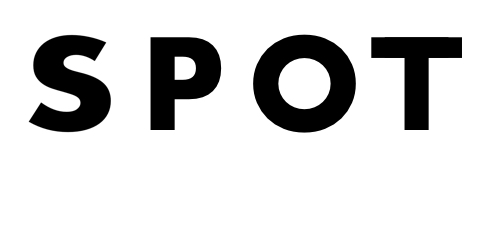
\includegraphics[width=0.6\linewidth]{figures/spot.pdf}
    \oscaption{spot}{%
        Time evolution of a Gaussian absorption line on a rigidly rotating, 
        spotted star computed from the analytic formulae in \S\ref{sec:kT}.
        The stellar surface is modeled as a spherical harmonic expansion
        up to $l=20$, and the line shape is assumed to be the same everywhere;
        the spot simply downweights the local intensity at all wavelengths.
        As the spot rotates into view (left panel), the line shape changes
        slightly (center panel). The residuals between the line when the
        spot is in view (solid) and when it is on the backside of the star
        (dotted) are shown in the right panel, where
        a Gaussian-like feature can be seen tracking the spot as it rotates
        from the blueshifted hemisphere to the redshifted hemisphere of
        the star.
        \label{fig:spot}
    }
    \end{centering}
\end{figure}

Figure~\ref{fig:compare} shows one of the spectra in Figure~\ref{fig:spot},
this time computed using both our formulae (blue line) and the traditional
technique of discretizing the stellar surface, Doppler-shifting the spectrum
in each grid cell according to the local radial velocity, interpolating back
to a uniform wavelength grid, and summing over the spatial dimension
(dotted orange line). We show the residuals in the lower panel, where it
is clear that as the number of grid cells increases from 2,000 (light grey)
to 71,000 (dark grey), the numerical solution approaches the solution
obtained using our approach. \xxx{Understand---and comment on---the fundamental
differences between a discrete linear convolution and traditional linear 
interpolation. Should we expect the numerical solution to actually \emph{converge}
to the \starry solution, or is the way the two are interpolating fundamentally
different?}

\begin{figure}[t!]
    \begin{centering}
    \includegraphics[width=0.65\linewidth]{figures/compare.pdf}
    \oscaption{compare}{%
        The observed spectrum when the spot is in view computed with
        \starry (blue) and numerically (orange). The problem setup
        is the same as that in Figure~\ref{fig:spot}. The bottom
        panel shows the absolute value of the difference between the 
        two spectra for different number of grid points in the 
        numerical solution.
        As the number of grid points increases, the numerical solution
        approaches the \starry solution.
        \label{fig:compare}
    }
    \end{centering}
\end{figure}


\section{Linearization}
\label{sec:linear}

\begin{figure}[ht!]
    \begin{centering}
    \includegraphics[width=0.8\linewidth]{figures/linalg.pdf}
    \oscaption{linalg}{%
        The Doppler design matrix $\Doppler$ (Equation~\ref{eq:linear:f}), 
        constructed from a grid of Toeplitz
        matrices, each of shape $K \times K'$, where $K$
        is the number of wavelength bins in the observed spectrum and
        $K' = K + W - 1$ is the number of bins in the model spectrum,
        where $W$ is the width of the convolution kernel.
        The $N$ columns of $\Doppler$ correspond
        to the Toeplitz matrices for each of the $N$ spherical harmonics
        (shown at the top);
        the $M$ rows correspond to the Toeplitz matrices rotated to each
        of the $M$ stellar phases observed (indicated graphically 
        to the left of $\Doppler$).
        \label{fig:linalg}
    }
    \end{centering}
\end{figure}

Although the convolution operator (Equation~\ref{eq:deconv:convolution_def})
is defined for continuous functions, the problem of Doppler imaging deals with
discrete measurements of a spectrum in bins of log wavelength. Provided our
wavelength grid is fine enough, we may therefore approximate 
Equation~(\ref{eq:deconv:convolution_def}) with a discrete convolution.
For discrete arrays $\bvec{g}$ and $\bvec{h}$, we have
%
\begin{align}
    \label{eq:linear:convolution_def}
    \bvec{g} * \bvec{h} = \bvec{G} \, \bvec{h}
\end{align}
%
where $\bvec{G}$ is a Toeplitz matrix, a matrix whose diagonals
are constant from top left to bottom right. In this case, the diagonals
are constructed from the values of $\bvec{g}$. If $\bvec{g}$ has length
$L$, element $g_n$ is placed everywhere along the $k^\mathrm{th}$ diagonal 
of $\bvec{G}$ for $k = -L / 2 + n$; all other entries of $\bvec{G}$ are 
set to zero. Note that the matrix $\bvec{G}$ need not be square; in fact,
for our purposes, it is a $(K \times K')$ matrix, where $K$ is the 
size of the observed wavelength grid and $K' = K + W - 1$ is the size of the
wavelength grid in the rest frame, where $W$ is the width of the convolution
kernel.

Given this formulation, we may re-write Equation~(\ref{eq:deconv:F}) as a
purely linear operation on $\azero(\lnlam_0)$:
%
\begin{align}
    \label{eq:linear:ft}
    \bvec{f}_t
    &=
    \Doppler_t
    \,
    \azero
    \quad,
\end{align}
%
where $\Doppler_t$ is a $(K \times N K')$ matrix constructed
by horizontally concatenating the Toeplitz matrices for each of the $N$ 
components of the convolution kernel $\kT(\lnlam, \Dargs)$ after rotating 
them (via $\R(t)$) to the stellar phase at time $t$. 
%
The $(K \times 1)$ vector $\mathbf{f}$ is the model for 
the flux observed at each wavelength at a particular time, and the 
$(N K' \times 1)$ vector $\azero$ is the vector representation of the
spatially-dependent spectrum of the star. The latter is constructed
by flattening the spherical harmonic expansion of the star
such that the first $K'$ terms in $\azero$ correspond
to the the values of $(a_0)_{0,0}$ at each wavelength $\lnlam_0$,
followed by the values of $(a_0)_{1,-1}$ at each wavelength, and so forth.

In general, our data will consist of observations made at several
epochs, corresponding to different rotational phases of the star. 
If we concatenate all $M$ spectra $\bvec{f}_t$ into the $(MK \times 1)$ 
vector $\bvec{f}$, we may write
%
\begin{align}
    \label{eq:linear:f}
    \bvec{f}
    &=
    \Doppler
    \,
    \azero
    \quad,
\end{align}
%
where $\Doppler$ is the full $(MK \times N K')$ Doppler design matrix, 
constructed by vertically concatenating the individual matrices $\Doppler_t$.
This equation represents the full linearization of the problem, where we
have expressed the quantity we can observe, $\bvec{f}$, as a linear
operation on the quantity of interest, the spectral/spatial decomposition
of the stellar surface, $\azero$. Figure~\ref{fig:linalg} shows an
example of $\Doppler$.

\section{The inverse problem}
\label{sec:inverse}
%
In the previous section we showed how to express the data vector $\bvec{f}$,
a series of spectra obtained at different epochs, as a purely linear
operation on the map vector $\azero$, the spherical harmonic decomposition of
the specific intensity on the surface of the star. The advantage of this
linearity is that, given suitable priors, it allows one to compute both 
the maximum likelihood solution for $\azero$ and its uncertainty
\emph{analytically}. In particular, if one places a (multidimensional)
Gaussian prior on $\azero$ with mean $\boldsymbol{\mu}_\mathbf{a_0}$ and 
covariance $\boldsymbol{\Lambda}_\mathbf{a_0}$, the maximum \emph{a posteriori} (MAP) 
solution for $\azero$ is
%
\begin{align}
    \label{eq:inverse:ahat}
    \bvec{\hat{a}_0} &= 
    \boldsymbol{\Sigma}_\mathbf{\hat{a}_0}
    \left(
        \Doppler^\top
        {\boldsymbol{\Sigma}_\mathbf{f}}^{-1}
        \bvec{f}
        +
        {\boldsymbol{\Lambda}_{\azero}}^{-1} \boldsymbol{\mu}_\mathbf{a_0}
    \right)
    \quad,
\end{align}
%
with posterior covariance given by
%
\begin{align}
    \label{eq:inverse:acov}
    \boldsymbol{\Sigma}_\mathbf{\hat{a}_0} &= 
    \left(
        \Doppler^\top
        {\boldsymbol{\Sigma}_\mathbf{f}}^{-1}
        \Doppler
        +
        {\boldsymbol{\Lambda}_{\azero}}^{-1}
    \right)^{-1}
    \quad,
\end{align}
%
where $\boldsymbol{\Sigma}_\mathbf{f}$ is the data covariance
matrix. These equations require the inversion of a few fairly
large matrices, but as we will see later, it allows one to obtain
the map of the star ($\bvec{\hat{a}_0}$) and its uncertainty
($\boldsymbol{\Sigma}_{\mathbf{\hat{a}_0}}$) in under a second for
a typical dataset.

There is, however, a catch: for most practical purposes, it is 
difficult to find a good Gaussian prior for $\bvec{a_0}$. Usually
we will have some prior information on what the spectrum of the
star is, and perhaps some prior information on the distribution
of surface features such as starspots. The problem is that
even if these priors are Gaussian, the corresponding prior
on $\bvec{a_0}$ is \emph{not}. To understand this, consider the
case where the stellar rest frame spectrum is spatially constant,
save for an amplitude that is spatially variable. We can then
describe the rest frame spectrum by the $(K' \times 1)$ vector
$\bvec{s}$ and the amplitude by the $(N \times 1)$ vector 
$\bvec{y}$ representing the spherical harmonic expansion of the
intensity profile of the star. The vector $\azero$ is then
given by the (flattened) outer product of the two vectors:
%
\begin{align}
    \label{eq:inverse:azero}
    \azero &= \mathrm{vec}\left( \bvec{A_0} \right) \nonumber \\
         &= \mathrm{vec}\left( \bvec{s} \, \bvec{y}^\top \right) \quad,
\end{align}
%
where $\mathrm{vec}$ denotes the vectorization operation, which in this case
transforms the $(K' \times N)$ matrix $\bvec{A_0}$ into the $(N K' \times 1)$
column vector $\azero$ by vertically stacking all of its columns. In other
words, the vector $\azero$ consists of the set of $K'$ intensities in
each wavelength bin repeated $N$ times, each time multiplied by the 
$n^\mathrm{th}$ spherical harmonic coefficient in the expansion of the 
surface intensity. Returning to our point about priors, note that all of the
entries of $\azero$ are the product of two independent random variables. Since
the product of two random variables is generally non-Gaussian, even
when the variables themselves are Gaussian%
\footnote{see, e.g., \url{http://mathworld.wolfram.com/NormalProductDistribution.html}}%
, so too is the prior on $\azero$. This point makes
Equation~(\ref{eq:inverse:ahat}) of little practical use, since a 
multivariate Gaussian will not 
generally be a suitable prior for $\azero$.

That said, a Gaussian prior \emph{is} typically suitable for both the spectrum
$\bvec{s}$ and the intensity $\bvec{y}$ (just not their product). It is
straightforward to show that because Equation~(\ref{eq:linear:f}) is linear
in $\azero$, it is also linear in both $\bvec{s}$ and $\bvec{y}$, so
MAP solutions can be found analytically for $\bvec{s}$ 
(conditioned on $\bvec{y}$) and $\bvec{y}$ (conditioned on $\bvec{s}$). We
investigate these solutions below.

\subsection{Solution for the intensity}
\label{sec:solve_y}
For a fixed, spatially constant rest-frame spectrum $\bvec{s}$, the model
for the flux vector may be written as
%
\begin{align}
    \label{eq:inverse:fy}
    \bvec{f}
    &=
    \Doppler
    \,
    \bvec{S}
    \,
    \bvec{y}
    \quad,
\end{align}
%
where
%
\begin{align}
    \setstackgap{L}{1.25\baselineskip}
    \bvec{S} =
        \begin{pmatrix}
        \quadquad\bvec{s}\quadquad & &            &            &  \\
        & \quadquad\bvec{s}\quadquad &            &            &  \\
        &            & \quadquad\bvec{s}\quadquad &            &  \\
        &            &            & \quadquad\bvec{s}\quadquad &  \\
        &            &            &               & \ddots
        \end{pmatrix}
\end{align}
%
is a $(NK' \times N)$ block matrix constructed by repeating the column
vector $\bvec{s}$ $N$ times in blocks along the main diagonal. 
%
Before we solve this equation for $\bvec{y}$, we note that in practice
it is convenient to fix the coefficient of the $Y_{0,0}$ spherical
harmonic, $y_0$, to unity. After all, this coefficient is not directly
constrained by the data, as it merely sets the baseline intensity on the
surface of the star and is therefore formally degenerate with the stellar 
luminosity (which also cannot be directly inferred from the data). This
choice further ensures a mean baseline of unity for the model 
vector $\mathbf{f}$. We may therefore write
%
\begin{align}
    \label{eq:inverse:fy1}
    \bvec{f}
    &=
    \Doppler
    \,
    \bvec{s}_\bvec{0}
    \,
    +
    \,
    \Doppler
    \,
    \bvec{S_1}
    \,
    \bvec{y}_\bvec{1}
    \quad,
\end{align}
%
where the vector $\bvec{s_0}$ denotes the first column of $\bvec{S}$,
the matrix $\bvec{S_1}$ denotes the remaining columns of $\bvec{S}$, and
$\bvec{y_1}$ is the quantity we wish to solve for: the vector of spherical 
harmonic coefficients of degree $l \ge 1$.

Given prior mean $\boldsymbol{\mu}_\bvec{y_1}$ and covariance
$\boldsymbol{\Lambda}_\bvec{y_1}$ on $\bvec{y_1}$, the MAP solution
is given by
%
\begin{align}
    \label{eq:inverse:y1hat}
    \bvec{\hat{y}_1} &= 
    \boldsymbol{\Sigma}_\mathbf{\hat{y}_1}
    \left(
        \bvec{S_1}^\top\Doppler^\top
        {\boldsymbol{\Sigma}_\mathbf{f}}^{-1}
        \left(\bvec{f} - \Doppler\bvec{s}_\bvec{0}\right)
        +
        {\boldsymbol{\Lambda}_\bvec{y_1}}^{-1} \boldsymbol{\mu}_\bvec{y_1}
    \right)
    \quad,
\end{align}
%
with covariance
%
\begin{align}
    \label{eq:inverse:y1cov}
    \boldsymbol{\Sigma}_\bvec{\hat{y}_1} &= 
    \left(
        \bvec{S_1}^\top\Doppler^\top
        {\boldsymbol{\Sigma}_\bvec{f}}^{-1}
        \Doppler\bvec{S_1}
        +
        {\boldsymbol{\Lambda}_\bvec{y_1}}^{-1}
    \right)^{-1}
    \quad.
\end{align}
%
If we choose a prior with zero mean ($\boldsymbol{\mu}_\bvec{y_1} = 0$)
and a diagonal covariance that is constant for each spherical harmonic 
order $m$,
%
\begin{align}
    \boldsymbol{\Lambda}_\bvec{y_1} &=
    \mathrm{diag} \left(
        \sigma_1^2
        \quad\quad\quad\quad
        \sigma_1^2
        \quad\quad\quad\quad
        \sigma_1^2
        \quad\quad\quad\quad
        \sigma_2^2
        \quad\quad\quad\quad
        \sigma_2^2
        \quad\quad\quad\quad
        \sigma_2^2
        \quad\quad\quad\quad
        \sigma_2^2
        \quad\quad\quad\quad
        \sigma_2^2
        \quad\quad\quad\quad
        \cdots
    \right)
    \quad,
\end{align}
%
we are in fact imposing an isotropic prior with an angular power spectrum
given by $C_l = \sigma_l^2$
\citep[e.g.,][]{Baldi2006}. This is especially useful if the typical
angular scale of features on the surface of the star is known or if
a Gaussian prior can be placed on it.

\subsection{Solution for the spectrum}
\label{sec:solve_s}
If, on the other hand, the spatial intensity profile is known, the
model for the flux vector may be written in terms of the spectrum $\bvec{s}$
as
%
\begin{align}
    \label{eq:inverse:fs}
    \bvec{f}
    &=
    \Doppler
    \,
    \bvec{Y}
    \,
    \bvec{s}
    \quad,
\end{align}
%
where
%
\begin{align}
    \setstackgap{L}{1.25\baselineskip}
    \bvec{Y} =
        \begin{pmatrix}
            y_0\, \bvec{I}_{K'} \\
            y_1\, \bvec{I}_{K'} \\
            y_2\, \bvec{I}_{K'} \\
            y_3\, \bvec{I}_{K'} \\
            \cdots
        \end{pmatrix}
\end{align}
%
is a $(NK' \times K')$ matrix constructed by vertically stacking
$N$ $(K' \times K')$ identity matrices, each multiplied by the
corresponding coefficient of $\bvec{y}$. Given
prior mean $\boldsymbol{\mu}_\mathbf{s}$ and covariance
$\boldsymbol{\Lambda}_\mathbf{s}$ on $\mathbf{s}$, the MAP solution
is given by
%
\begin{align}
    \label{eq:inverse:shat}
    \bvec{\hat{s}} &= 
    \boldsymbol{\Sigma}_\mathbf{\hat{s}}
    \left(
        \bvec{Y}^\top\Doppler^\top
        {\boldsymbol{\Sigma}_\mathbf{f}}^{-1}
        \bvec{f}
        +
        {\boldsymbol{\Lambda}_\mathbf{s}}^{-1} \boldsymbol{\mu}_\mathbf{s}
    \right)
    \quad,
\end{align}
%
with covariance
%
\begin{align}
    \label{eq:inverse:scov}
    \boldsymbol{\Sigma}_\mathbf{\hat{s}} &= 
    \left(
        \bvec{Y}^\top\Doppler^\top
        {\boldsymbol{\Sigma}_\mathbf{f}}^{-1}
        \Doppler\bvec{Y}
        +
        {\boldsymbol{\Lambda}_\mathbf{s}}^{-1}
    \right)^{-1}
    \quad.
\end{align}

\subsection{The full solution}
In the previous two sections we showed how, if the stellar
rest-frame spectrum is spatially constant and known \emph{a priori} 
(from, say, a template spectrum), the posterior distribution
for the surface map $\bvec{y}$ is \emph{analytic} 
(Equations~\ref{eq:inverse:y1hat}
and \ref{eq:inverse:y1cov}). Conversely, if the surface map is known,
the posterior for the spectrum is also analytic 
(Equations~\ref{eq:inverse:shat} and \ref{eq:inverse:scov}). Both sets of
solutions require Gaussian priors on the quantities of interest, but these
are easily interpretable. A Gaussian prior on
the spherical harmonic coefficients of the surface map corresponds 
to the angular power spectrum of the surface features, whereas a Gaussian
prior on the spectrum can be used to correctly propagate uncertainties in
the stellar spectrum from observational uncertainties on the stellar
metallicity, temperature, etc.

Importantly, the framework developed here allows one to analytically
compute not only the ``optimal'' solution to the Doppler imaging problem,
but also its uncertainty. The problem of re-constructing surface images
of stars from spectra and/or light curves is fundamentally ill-posed because
of intrinsic degeneracies and a large null space
\citep[e.g.,][]{Luger2019} \xxx{more cites}. Coupled to uncertainties in
the observations themselves, this makes the process of searching for the
``optimal'' solution flawed at best, and meaningless at worst. Access to the
full covariance matrix of the solution is therefore essential to assessing our
confidence in the various features of the inferred surface maps.

However, as we mentioned above, the Doppler imaging problem can be solved
analytically for either the surface map or the spectrum, but not both. If
neither are known exactly \emph{a priori}, which is quite often the case,
we can still find the MAP solution quickly by guessing at an initial
spectrum $\bvec{s}$ and iterating between optimizing for $\bvec{y}$ and
optimizing for $\bvec{s}$. This bi-linear problem is not generally convex,
but given a good starting point for $\bvec{s}$ and sufficient regularization
on $\bvec{y}$, we find that it typically converges to the correct solution,
especially after refinement with a non-linear solver;
we discuss this in detail below.

Once the MAP solution has been found for both $\bvec{s}$ and $\bvec{y}$,
the covariance of one conditioned on the other can be computed from the
formulae above. However, this is necessarily a lower bound on the true
covariance of the solution, since it neglects any covariance \emph{between}
$\bvec{s}$ and $\bvec{y}$. To \emph{correctly} account for this, one must
resort to Monte Carlo methods or other sampling techniques. We discuss
this further below.


\section{Bells and Whistles}
\label{sec:bells}

\subsection{Unknown continuum normalization}
\label{sec:norm}
%
Consider the star depicted in Figure~\ref{fig:spot}. When the spot is in
view, absorption lines become distorted due to the suppression of either
blueshifted or redshifted light. However, what is not shown in the figure
is the fact that overall, the star also gets \emph{dimmer}: the 
continuum level drops in the presence of the spot. Unfortunately, 
spectrographs are not usually designed to measure this, since the
change in the star's overall brightness from one observation to the next
is often dwarfed by (unknown) changes in the spectrograph sensitivity. 
For this reason, the spectra are usually normalized to have a
fixed baseline continuum, and Equation~\ref{eq:linear:f} is no longer
a good model for the data.

One option is to collect simultaneous photometry on the target in a band
similar to the wavelength range observed, and use this light curve to
(un-)normalize the spectral timeseries $\bvec{f}$. However, when this is
not an option, our model for $\bvec{f}$ (Equation~\ref{eq:linear:f}) must
be amended.

%
\begin{align}
    \label{eq:norm:f}
    \bvec{f}
    &=
    \frac{
        \Doppler
        \,
        \azero
    } {
        \bvec{b}
    }
    \quad,
\end{align}
%
where $\bvec{b}$ is the baseline and the vector division is
performed elementwise. When $\azero$ is given by Equation~(\ref{eq:inverse:azero}),
the baseline $\bvec{b}$ is simply the total (wavelength-integrated) flux
at each epoch, repeated for every element in each spectrum. 
Based on \citet{Luger2019}, this can be computed as a purely linear operation 
on the spherical harmonic vector $\bvec{y}$:
%
\begin{align}
    \label{eq:norm:b}
    \bvec{b}
    &=
    %
    \begin{pmatrix}
        \bvec{r}^\top \bvec{A_1} \bvec{R}(t_0) \\
        \cdots \\
        \bvec{r}^\top \bvec{A_1} \bvec{R}(t_0) \\
        \bvec{r}^\top \bvec{A_1} \bvec{R}(t_1) \\
        \cdots \\
        \bvec{r}^\top \bvec{A_1} \bvec{R}(t_1) \\
        \cdots \\
        \bvec{r}^\top \bvec{A_1} \bvec{R}(t_{M-1}) \\
        \cdots \\
        \bvec{r}^\top \bvec{A_1} \bvec{R}(t_{M-1})
    \end{pmatrix}
    \bvec{y}
    %
    \nonumber \\[0.5em]
    &\equiv
    \bvec{B} \, \bvec{y}
\end{align}
%
where $\bvec{r}$ is given by Equation~(18) in \citet{Luger2019},
$\bvec{A_1}$ is given in Appendix B of \citet{Luger2019}, and $\bvec{R}(t)$
is the rotation matrix defined previously.

Given this new equation, we must change how we approach the inverse problem
(\S\ref{sec:inverse}). When solving for the spectrum given the spherical 
harmonic vector (\S\ref{sec:solve_s}), we need only make the replacements
$\bvec{f} \rightarrow \nicefrac{\bvec{f}}{\bvec{B}\, \bvec{y}}$
and 
$\boldsymbol{\Sigma}_\mathbf{f} \rightarrow \nicefrac{\boldsymbol{\Sigma}_\mathbf{f}}{(\bvec{B}\, \bvec{y})^2}$ 
in Equations~(\ref{eq:inverse:shat}) and (\ref{eq:inverse:scov}).
However, when solving for the spherical harmonic vector given the spectrum
(\ref{sec:solve_y}), the problem is no longer linear in $\bvec{y}$, as the
vector of interest appears in both the numerator and the denominator:
%
\begin{align}
    \label{eq:norm:fy}
    \bvec{f}
    &=
    \frac{
        \bvec{D}
        \,
        \bvec{S}
        \,
        \bvec{y}
    }{
        \bvec{B}
        \,
        \bvec{y}
    }
    \quad.
\end{align}
%
While we can solve for $\bvec{y}$ using a non-linear optimizer, it is
often the case that the denominator in Equation~(\ref{eq:norm:fy}) is close
to unity; i.e., the total flux from the star typically varies by only a
few percent. When this is the case, it is straightforward to linearize
this equation.
Following the notation from \S\ref{sec:solve_y}, we may therefore write
%
\begin{align}
    \bvec{f}
    &=
    \frac{
        \bvec{D} \, \bvec{s_0}
        \,
        + 
        \,
        \bvec{D}\bvec{S_1}
        \,
        \bvec{y_1}
    }{
        \bvec{B_0}
        \,
        +
        \bvec{B_1}
        \,
        \bvec{y_1}
    }
    \quad,
\end{align}
%
where $\bvec{B_0} = \bvec{1}$ is the first column of $\bvec{B}$
and $\bvec{B}_\bvec{1}$ denotes the
matrix composed from the remaining $N - 1$ columns of $\bvec{B}$.
Expanding the expression above about 
$\bvec{B_1} \bvec{y_1} = \bvec{0}$, we have
%
\begin{align}
    \label{eq:norm:fapprox}
    \bvec{f}
    &\approx
    \left(
        \bvec{D} \, \bvec{s_0}
        \,
        + 
        \,
        \bvec{D}\bvec{S_1}
        \,
        \bvec{y_1}
    \right)
    \circ
    \left(
        \bvec{1}
        \,
        -
        \bvec{B_1}
        \,
        \bvec{y_1}
    \right)
    \nonumber \\
    &=
    \left(
        \bvec{D}\bvec{S_1}
        \,
        -
        \bvec{C}
    \right)
    \bvec{y_1}
    \,
    +
    \,
    \bvec{D} \, \bvec{s_0}
    \quad,
\end{align}
%
where $\circ$ denotes an elementwise product and $\bvec{C}$ is a matrix
constructed by multiplying the $i^\mathrm{th}$ row of $\bvec{B_1}$ by the
$i^\mathrm{th}$ element of $\bvec{D}\bvec{s_0}$.
%
This equation is now
linear in $\bvec{y}_\bvec{1}$, so we may solve the least-squares problem
as before:
%
\begin{align}
    \label{eq:norm:yhat}
    \bvec{\hat{y}_1} &= 
    \boldsymbol{\Sigma}_\mathbf{\hat{y}_1}
    \left(
        \left(\bvec{D}\bvec{S_1} - \bvec{C}\right)^\top
        {\boldsymbol{\Sigma}_\mathbf{f}}^{-1}
        (\bvec{f} - \bvec{D}\bvec{s_0})
        +
        {\boldsymbol{\Lambda}_{\mathbf{y}_\bvec{1}}}^{-1} \boldsymbol{\mu}_{\mathbf{y}_\bvec{1}}
    \right)
    \quad,
\end{align}
%
with covariance
%
\begin{align}
    \label{eq:norm:ycov}
    \boldsymbol{\Sigma}_\mathbf{\hat{y}_1} &= 
    \left(
        \left(\bvec{D}\bvec{S_1} - \bvec{C}\right)^\top
        {\boldsymbol{\Sigma}_\mathbf{f}}^{-1}
        \left(\bvec{D}\bvec{S_1} - \bvec{C}\right)
        +
        {\boldsymbol{\Lambda}_{\mathbf{y}_1}}^{-1}
    \right)^{-1}
    \quad.
\end{align}
%
Note, importantly, that these equations are valid only in the limit that the
change in the total flux from the star is small. Nevertheless, even in the 
general case, we find that solving this linear problem yields a good
starting point for a non-linear optimization, which we revisit in more
detail below.

\subsection{Limb darkening}
Hello.

\subsection{Multiple spectra}
Hello.

\section{The SPOT star}
\label{sec:spotstar}

\cite{Vogt1987}

\begin{figure}[p!]
    \begin{centering}
    \includegraphics[width=0.49\linewidth]{figures/spot_y1_timeseries.pdf}
    \includegraphics[width=0.49\linewidth]{figures/spot_y1_rect.pdf}
    \oscaption{spot_y1}{%
        Solution to the \spot problem at high SNR when both 
        the rest frame spectrum and the baseline are known.
        \label{fig:spot_y1}
    }
    \end{centering}
\end{figure}

\begin{figure}[p!]
    \begin{centering}
    \includegraphics[width=0.49\linewidth]{figures/spot_y1b_timeseries.pdf}
    \includegraphics[width=0.49\linewidth]{figures/spot_y1b_rect.pdf}
    \\[0.5em]
    \includegraphics[width=0.405\linewidth]{figures/spot_y1b_baseline.pdf}
    \includegraphics[width=0.575\linewidth]{figures/spot_y1b_coeffs.pdf}
    \oscaption{spot_y1b}{%
        Similar to Figure~\ref{fig:spot_y1}, but assuming the baseline
        is not known.
        \label{fig:spot_y1b}
    }
    \end{centering}
\end{figure}

\begin{figure}[p!]
    \begin{centering}
    \includegraphics[width=0.49\linewidth]{figures/spot_y1bs_timeseries.pdf}
    \includegraphics[width=0.49\linewidth]{figures/spot_y1bs_rect.pdf}
    \\[0.5em]
    \includegraphics[width=0.405\linewidth]{figures/spot_y1bs_baseline.pdf}
    \includegraphics[width=0.575\linewidth]{figures/spot_y1bs_coeffs.pdf}
    \\[0.5em]
    \includegraphics[width=0.98\linewidth]{figures/spot_y1bs_spectrum.pdf}
    \oscaption{spot_y1bs}{%
        Similar to Figure~\ref{fig:spot_y1}, but assuming we have no
        information about either the spectrum, the baseline, or the map
        coefficients.
        \label{fig:spot_y1bs}
    }
    \end{centering}
\end{figure}

\begin{figure}[h!]
    \begin{centering}
    \includegraphics[width=0.98\linewidth]{figures/inclinations.pdf}
    \oscaption{inclinations}{%
        Recovered \spot map as a function of inclination.
        \label{fig:inclinations}
    }
    \end{centering}
\end{figure}

\section{Performance}
\label{sec:performance}

Evaluation of the model via Equation~(\ref{eq:deconv:F}) requires 
first the rotation of the $(\lmax + 1)^2$
$\kT$ kernels (each of length $W$) to the correct stellar 
rotational phase, an operation that scales approximately
as $W \lmax^3$,
followed by $(\lmax + 1)^2$
linear convolutions of the rotated $\kT$ kernels with the 
spectral components (each of length $K$), which scales
approximately as $W K \lmax^2$. Since typically $K \gg \lmax$,
the latter computation dominates and the entire evaluation 
takes $\mathcal{O}(W K \lmax^2)$ operations.

\section{Stuff we're not addressing}
%
Differential rotation and convective blueshift.

%
%
%
%
\clearpage
\appendix
%
%
%
%

\section{Solving the $\kT$ integral}
%
In this section we will show how to compute the integral in
Equation~(\ref{eq:kT:kT}), yielding the terms of the convolution
kernel $\kT$. It is convenient to first change basis from spherical harmonics to 
polynomials on the sphere:
%
\begin{align}
    \label{eq:appendix:kT}
    \kT(\lnlam, \Dargs) 
    &=    
    \int\limits_{-\sqrt{1 - x^2}}^
                {\sqrt{1 - x^2}}
    \pbasis
    \Big(x, y\Big)
    \mathrm{d}y
    \,
    \AOne
    \nonumber \\[0.5em]
    &\equiv
    \rhoT(\lnlam, \Dargs) 
    \,
    \AOne
    \quad,
\end{align}
%
where $\AOne$ is the change of basis matrix from spherical harmonics
to polynomials \citep[Equation B11 in][]{Luger2019} and
%
\begin{align}
    \pbasis(\x) \equiv 
\Big( 
    1 \quad\quad\quad\quad\quad\quad 
    x \quad\quad\quad\quad\quad\quad 
    z \quad\quad\quad\quad\quad\quad 
    y \quad\quad\quad\quad\quad\quad 
    x^2 \quad\quad\quad\quad\quad\quad 
    xz \quad\quad\quad\quad\quad\quad 
    xy \quad\quad\quad\quad\quad\quad
    yz \quad\quad\quad\quad\quad\quad 
    y^2 \quad\quad\quad\quad\quad\quad
    ... 
\Big)^\top
\quad,
\end{align}
%
is the polynomial basis \citep[Equation 7][]{Luger2019}. 
The $n^\mathrm{th}$ term of the polynomial basis
is a polynomial in $x$, $y$, and $z = \sqrt{1 - x^2 - y^2}$:
%
\begin{proof}{PolynomialBasis}
    \pbasisn
    &=
    x^i y^j z^k
\end{proof}
%
where $i, j, k$ are integers given by
%
\begin{proof}{PolynomialBasis}
    \label{eq:kT:lm}
    i &= \floor*{\Lambda - \Delta}
    \nonumber \\[0.5em]
    j &= \floor*{\Delta}
    \nonumber \\[0.5em]
    k &= \ceil*{\Delta} - \floor*{\Delta}
\end{proof}
%
with
%
\begin{proof}{PolynomialBasis}
    \Lambda &= \floor*{\sqrt{n}}
    \nonumber \\[0.5em]
    \Delta &= \frac{n - \Lambda^2}{2}
    \quad .
\end{proof}
%
We may now explicitly write down the $n^\mathrm{th}$ term of 
the vector $\rhoT(\lnlam, \Dargs)$ in Equation~(\ref{eq:appendix:kT}),
%
\begin{align}
    \label{eq:kT:sTexpression}
    \rho_n(\lnlam, \Dargs) 
    &=    
    \rho_{i,\,j,\,k}(\lnlam, \Dargs) 
    =    
    x^i
    \int\limits_{-\sqrt{1 - x^2}}^
                {\sqrt{1 - x^2}}
        y^j
        \left(1 - x^2 - y^2\right)^{\frac{k}{2}} \,
    \mathrm{d}y 
    \quad .
\end{align}
%
When $i = k = 0$, the integral is easy to evaluate:
%
\begin{align}
    \rho_{i,\,j,\,0}(\lnlam_0) 
    &=    
    \begin{cases}
        2 \left( 1 - x^2 \right)^\frac{j + 1}{2} 
        \quad\quad\quad\quad\quad\quad\quad\quad\quad\quad\quad\quad 
        &  j \, \mathrm{even} \\
        0 & j \, \mathrm{odd} \quad .
    \end{cases}
\end{align}
%
The general term may be computed from the recurrence relation
%
\begin{align}
    \rho_{0,\,j,\,0}(\lnlam_0) = \frac{j - 1}{j + 1} \big(1 - x^2\big) \rho_{0,\,j-2,\,0}
\end{align}
%
provided 
%
\begin{align}
    \rho_{0,\,0,\,0} &= 2 \sqrt{1-x^2} \nonumber \\
    \rho_{0,\,1,\,0} &= 0 \quad.
\end{align}
%
When $i = 0$ and $k = 1$, we may substitute $y = \sin\psi\sqrt{1 - x^2}$ in
the integrand to obtain
%
\begin{align}
    \rho_{0,\,j,\,1}(\lnlam_0)
    &=
    (1 - x^2)^{\frac{j + 2}{2}}
    \int\limits_{-\frac{\pi}{2}}^{\frac{\pi}{2}}
        \sin^j\psi
        \cos^2\psi \,
    \mathrm{d}\psi
    \quad.
\end{align}
%
We may solve this integral using the recurrence relation
%
\begin{align}
    \int
        \sin^j\psi
        \cos^m\psi \,
    \mathrm{d}\psi
    &=
    -\frac{\sin^{j-1}\psi \cos^{m+1}\psi}{j + m}
    +
    \frac{j - 1}{j + m}\int\sin^{j-2}\psi \cos^m\psi \mathrm{d}\psi
    \quad ,
\end{align}
%
which, in our case, simplifies to
%
\begin{align}
    \int\limits_{-\frac{\pi}{2}}^{\frac{\pi}{2}}
        \sin^j\psi
        \cos^2\psi \,
    \mathrm{d}\psi
    &=
    \frac{j - 1}{j + 2}\int\limits_{-\frac{\pi}{2}}^
        {\frac{\pi}{2}}\sin^{j-2}\psi \cos^2\psi \mathrm{d}\psi
    \quad.
\end{align}
%
We thus arrive at the recurrence relation
%
\begin{align}
    \rho_{0,\,j,\,1} &= \frac{j - 1}{j + 2} \big(1 - x^2\big) \rho_{0,\,j-2,\,1}
\end{align}
%
with initial conditions
%
\begin{align}
    \rho_{0,\,0,\,1} &= \frac{\pi}{2} \big(1-x^2\big) \nonumber \\
    \rho_{0,\,1,\,1} &= 0 \quad.
\end{align}
%
Given these expressions, recursing upward in $i$ is easy:
%
\begin{align}
    \rho_{i,\,j,\,k} &= x \, \rho_{i-1,\,j,\,k} \quad.
\end{align}
%
This completes our derivation. To summarize, given the boundary conditions
%
\begin{align}
    \rho_{0,\,0,\,0} &= 2 \sqrt{1-x^2} \nonumber \\
    \rho_{0,\,0,\,1} &= \frac{\pi}{2} \big(1-x^2\big) \nonumber \\
    \rho_{0,\,1,\,k} &= 0 \quad ,
\end{align}
%
we may compute any term in $\rhoT$ via the expressions
%
\begin{align}
    \label{eq:kT:sTrecurrence}
    \rho_{0,\,j,\,k} &= \frac{j - 1}{j + 1 + k} \big(1 - x^2\big) \rho_{0,\,j-2,\,k} \nonumber \\
    \rho_{i,\,j,\,k} &= x \, \rho_{i-1,\,j,\,k} \quad.
\end{align}
%
The terms of the convolution kernel $\kT$ are then obtained by dotting
this vector into the change of basis matrix $\AOne$, as discussed above.

% Bibliography
\bibliography{bib}

\end{document}
